\documentclass{article}
\usepackage[utf8]{inputenc}
\usepackage{hyperref}
\hypersetup{
	colorlinks,
	citecolor=black,
	filecolor=black,
	linkcolor=black,
	urlcolor=black
}
\usepackage{graphicx}
\usepackage{amssymb}
\usepackage[fleqn]{amsmath}
\usepackage{pgfplots}
\usepackage{mathtools}
\usepackage[thinc]{esdiff}
\def\pgfplots@stacked@diff{}
\setlength\parindent{12pt}
\usepackage{tabularx}
\usepackage{makecell}

\DeclarePairedDelimiter\set\{\}


\title {Mathematical Methods 3/4 Bound Reference}
\author {Samuel Murphy}
\date{2023}

\pgfmathdeclarefunction{CubeRoot}{1}{%
	\pgfmathparse{ifthenelse(#1<0,-1,1)*exp((ln(abs(#1)))/3)}%
}

\begin{document}
	\maketitle
	\newpage
	\tableofcontents
	\newpage
	\section{AOS1 - Functions, Relations, and Graphs}
		\subsection{Distinguishing between a Function and Relation}
			\subsubsection{Relations}
				A relation is a set of ordered pairs $(x_1,y_1), (x_2,y_2)$ etc.\newline
				
		\subsection{Key Features and Properties of a Function or Relation}
			\subsubsection{Set Notation}
				Set notation is used to state/specify the domain and range of functions and relations.\newline
				\[A\subseteq B\text{; A is a subset of B, i.e. all values in A are contained in B} \]
				\[B\setminus A\text{; all values that are in set B but not set A}\]
				\[A \cup B\text{; all the values in A \textbf{or} B}\]
				\[A \cap B\text{; al the values in A \textbf{and} B}\]
				\textbf{Common Sets}\newline
				$\mathbb{R}$ = real numbers = all numbers over the interval $(-\infty,\infty)$ both rational and irrational.\newline
				$\mathbb{Q}$ = rational numbers = all real numbers that can be represented as a fraction. \newline
				$\mathbb{Z}$ = integers = all whole numbers \newline
				$\mathbb{N}$ = natural numbers = positive integers \newline
				$\mathbb{N}\subseteq\mathbb{Z}\subseteq\mathbb{Q}\subseteq\mathbb{R}$.
			\subsubsection{Interval Notation}
				\[x\in\mathbb{R}^+ = [0,\infty) = \{x:0\le x<\infty\}\]
				[ means an endpoint is included in the interval.\newline
				( means an endpoint is not included in the inteval.\newline
			\subsubsection{Stationary Points of Inflection}
				Stationary points of inflection are points of inflection at which the tangent line at that point has a gradient of 0.
			
				\begin{center}
					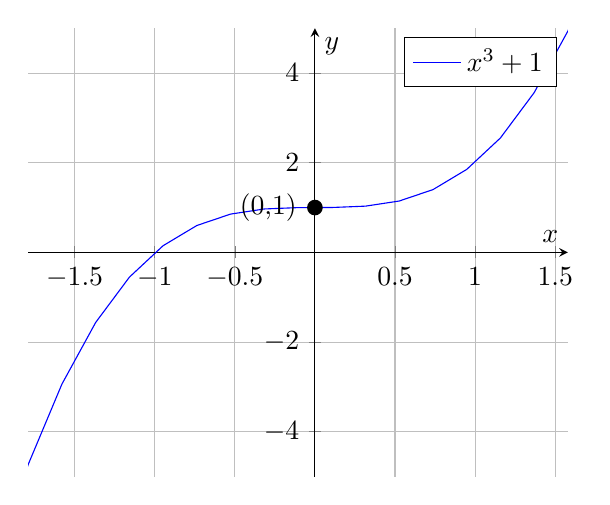
\begin{tikzpicture}
						\begin{axis} [
								axis lines=middle, 
								grid, 
								domain=-2:2,
								ymax=5, 
								ymin=-5, 
								xlabel={$x$}, 
								ylabel={$y$}
							]
							
							\addplot [
								color=blue, 
								samples=20 ]
								{x^3 + 1};
							
							\addlegendentry{$x^3 + 1$};
								
							\node [
								label={180:{(0,1)}},
								circle,
								fill,
								inner sep=2pt]
								at (axis cs:0,1)
							{};
						\end{axis}
					\end{tikzpicture}
				\end{center}
			
			\subsubsection{Non-stationary Points of Inflection}
				Non-stationary points of inflection are points of inflection at which the tangent line at that point has a non-zero gradient.
				\begin{center}
					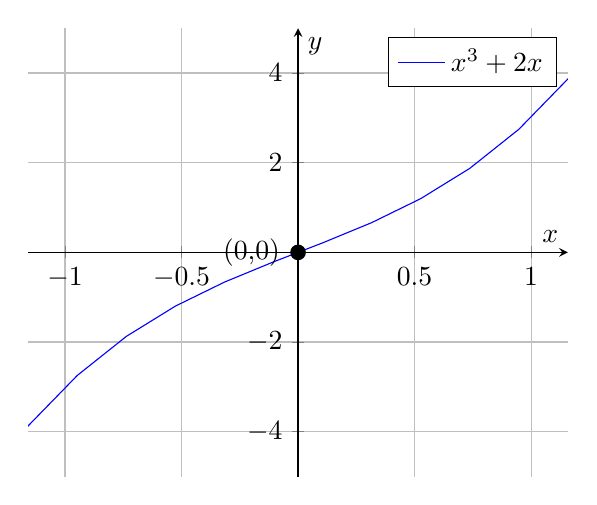
\begin{tikzpicture}
						\begin{axis} [
								axis lines=middle, 
								grid, 
								domain=-2:2,
								ymax=5, 
								ymin=-5, 
								xlabel={$x$}, 
								ylabel={$y$}
							]
							
							\addplot [
								color=blue, 
								samples=20 ] 
								{x^3 + 2*x};
							
							\addlegendentry{$x^3 + 2x$};
								
							\node [
								label={180:{(0,0)}},
								circle,
								fill,
								inner sep=2pt ]
								at (axis cs: 0,0)
							{};
						\end{axis}
					\end{tikzpicture}
				\end{center}
			\newpage
			\subsubsection{Symmetry of Functions - Even Functions}
				A function is called 'even' if it is symmetrical around the y-axis. $f(x)=f(-x)$ for all values of x.
				\begin{center}
					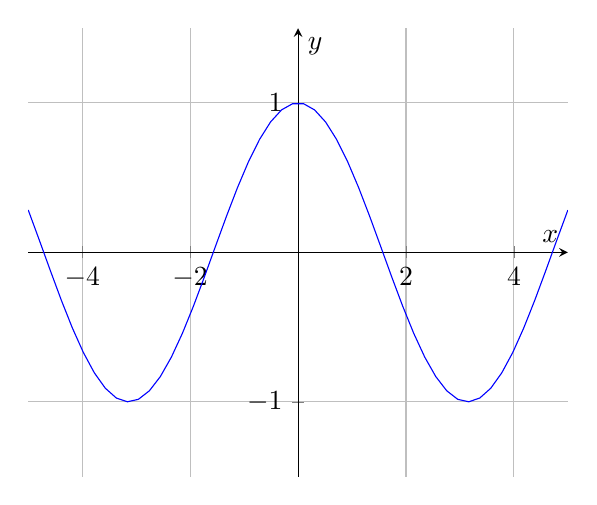
\begin{tikzpicture}
						\begin{axis} [
								axis lines=middle, 
								grid, 
								domain=-5:5,
								ymax=1.5, 
								ymin=-1.5, 
								xlabel={$x$}, 
								ylabel={$y$}
							]
							\addplot [
								color=blue,
								samples=50 ]
								{cos(deg(x))};
						\end{axis}
					\end{tikzpicture}
				\end{center}
			\subsubsection{Symmetry of Functions - Odd Functions}
				A function is called 'odd' if it is symmetrical about the origin. $f(x)=-f(-x)$ for all values of x.
				\begin{center}
					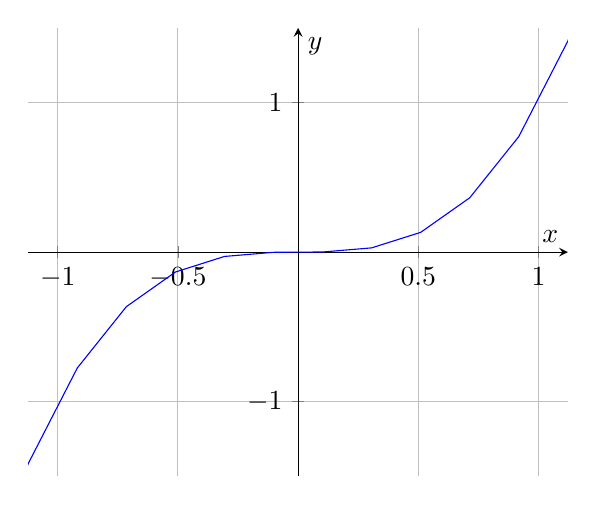
\begin{tikzpicture}
						\begin{axis} [
							axis lines=middle, 
							grid, 
							domain=-5:5,
							ymax=1.5, 
							ymin=-1.5, 
							xlabel={$x$}, 
							ylabel={$y$}
							]
							\addplot [
							color=blue,
							samples=50 ]
							{x^3};
						\end{axis}
					\end{tikzpicture}
				\end{center}
			\subsubsection{Symmetry of Polynomials}
				\begin{tabular}{|p{3cm}|p{10cm}|}
					\hline
					Even function & $f(x)=ax^4 + cx^2 + e$ about $x=0$. $(0,e)$ will be a turning point of the quartic. \\
					\hline
					Odd function & $f(x)=bx^3 + dx$ about $(0,0)$. $(0,0)$ is the point of inflection of the cubic. \\
					\hline\hline
					Reflective symmetry & $f(x)=a(x-h)^4+c(x-h)^2+e$ about $x=h$. $(h,e)$ will be a turning point of the quartic. \\
					\hline
					Rotational symmetry & $f(x)=b(x-h)^3+d(x-h)+e$ about $(h,e)$. $(h,e)$ is the point of inflection of the cubic.\\
					\hline
				\end{tabular}
			\subsubsection{Features of Sine and Cosine Functions}
				\[y=a\sin(nx)+c\;\;\text{and}\;\;y=a\cos(nx)+c\]
				\textbf{Amplitude}\newline
				The amplitude is the maximum displacement of a sine or cosine function from the mean value. It is the value of $a$, regardless of its sign. That is, $y=2\sin(x)$ and $y=-2\sin(x)$ both have an amplitude of 2.
				\newline\newline
				\textbf{Period}
				The domain of a single repetition of the function. For sine and cosine, this is given by $\frac{2\pi}{n}$. The value of $n$ also represents the number of cycles that can be fit into the original period of the function.
				\newline\newline
				\textbf{Mean Value}\newline
				The centre of a circular function. A sine or cosine function will oscillate about this value, and it is given by the value of $c$.
				\newline\newline
				\textbf{Maximums and Minimums}\newline
				Sine and cosine have maximum values of +1 and minimum values of -1. These will be changed under transformations. Maximum = mean position + amplitude and Minimum = mean position - amplitude.
		\subsection{Types of Function}
			\subsubsection{Natural Power Functions}
				\[f(x)=a[b(x-h)]^n - k\]
				\textbf{Positive Even \boldmath$n$; Turning-point Form}\newline
				For even powers of $x$, such as $y=x^2$ and $y=x^4$, the values of $y$ are the same for positive and negative values of $x$. That is $x^2=(-x)^2$. Therefore, reflectional symmetry occurs about $x=0$.\newline
				\textit{Quadratic}
				\[f(x)=x^2\;\;\mathbf{or}\;\;f(x)=a(x-h)^2+k\;\;\;\;\mathbf{Turning\;Point\;at}\;(h,k)\]
				\textit{Quartic}
				\[f(x)=x^4\;\;\mathbf{or}\;\;f(x)=a(x-h)^4+k\;\;\;\;\mathbf{Turning\;Point\;at}\;(h,k)\]
				\newline
				\textbf{Positive Odd \boldmath$n$; Point of Inflection Form}\newline
				For odd powers of $x$, such as $y=x$ and $y=x^3$, the values of $y$ are opposite for positive and negative values of $x$. That is, $-x^3=(-x)^3$. Therefore, there is rotational (180$\deg$ turn) symmetry about $(0,0)$.\newline
				\textit{Linear}
				\[f(x)=x\;\;\mathbf{or}\;\;f(x)=a(x-h)+k\;\;\;\;\mathbf{Point\;on\;line\;at}\;(h,k)\]
				\textit{Cubic}
				\[f(x)=x^3\;\;\mathbf{or}\;\;f(x)=a(x-h)^3+k\;\;\;\;\mathbf{Point\;of\;Inflection\;at}\;(h,k)\]
			\newpage
			\subsubsection{Negative Power Functions}
				\[f(x)=a[b(x-h)]^{-n}+k=\frac{a}{[b(x-h)]^n}+k\]
				Negative power functions have \textbf{asymptotes}. These are lines which the graph will approach but never reach. \newline
				The vertical asymptote of a negative power function is at $x=h$. Therefore, the \textbf{maximal domain} of a negative power function is $\mathbb{R} \setminus \{h\}$\newline\newline
				The \textbf{range} depends on if its an \textbf{even} or \textbf{odd} negative power function. Negative odd power functions have a range of $\mathbb{R} \setminus \{k\}$, whereas negative even power functions have a range of $(k,\infty)$ for $a>0$ or $(-\infty,k)$ for $a<0$.\newline\newline
				\textbf{Hyperbola (Odd negative power functions)}\newline
				$f(x)=x^{-1}=\frac{1}{x}$ forms the shape of a hyperbola.
				\begin{center}
					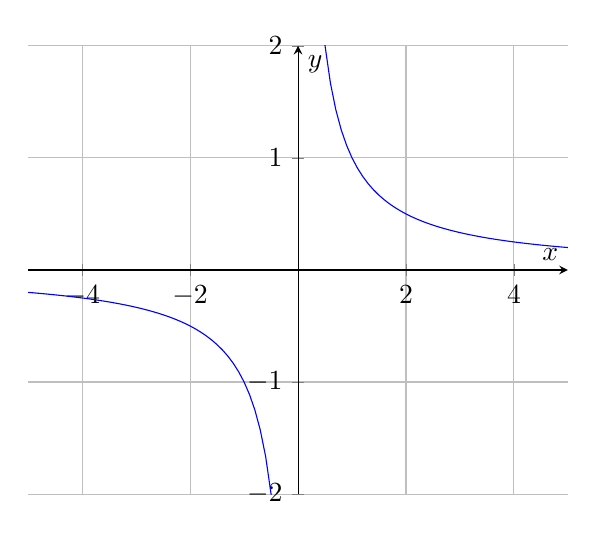
\begin{tikzpicture}
						\begin{axis} [
							axis lines=middle, 
							grid, 
							domain=-5:5,
							ymax=2, 
							ymin=-2, 
							xlabel={$x$}, 
							ylabel={$y$}
							]
							\addplot [
								color=blue,
								samples=101,
								unbounded coords=jump
							] {x^(-1)};
						\end{axis}
					\end{tikzpicture}
				\end{center}
				\[f(x)=\frac{a}{x-h}+k\;\;\textrm{shows the transformation of a hyperbola.}\]
				The equation of a hyperbola can also be written as $y=\frac{ax+b}{cx+d}$. In these cases, the numerator should be divided by the denominator to be written as $y=\frac{A}{x+B}+C$ to allow easier sketching.
				\newpage
				\noindent\textbf{Truncus (Even negative power functions)}\newline
				$f(x)=x^{-2}=\frac{1}{x^2}$ forms the shape of a truncus.
				\begin{center}
					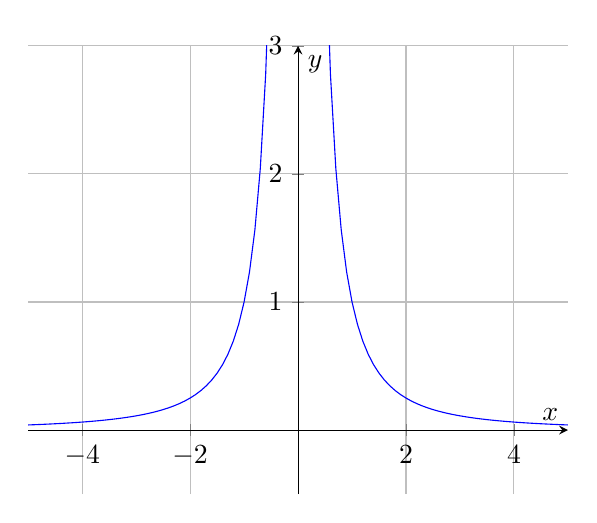
\begin{tikzpicture}
						\begin{axis} [
							axis lines=middle, 
							grid, 
							domain=-5:5,
							ymax=3, 
							ymin=-0.5, 
							xlabel={$x$}, 
							ylabel={$y$}
							]
							\addplot [
								color=blue,
								samples=101,
								unbounded coords=jump
							] {x^(-2)};
						\end{axis}
					\end{tikzpicture}
				\end{center}
				\[f(x)=\frac{a}{(x-h)^2}+k\;\;\textrm{shows the transformation of a truncus.}\]
				\newline
			\subsubsection{Root Funtions}
				\[f(x)=a[b(x-h)]^{\frac{1}{n}}+k=a\sqrt[n]{b(x-h)}+k\]
				\textbf{Square Root Function}
				\[f(x)=\sqrt{x}\;\;\mathbf{or}\;\;f(x)=a\sqrt{x-h}+k\;\;\;\;\mathbf{Endpoint\;at\;}(h,k)\]
				\begin{center}
					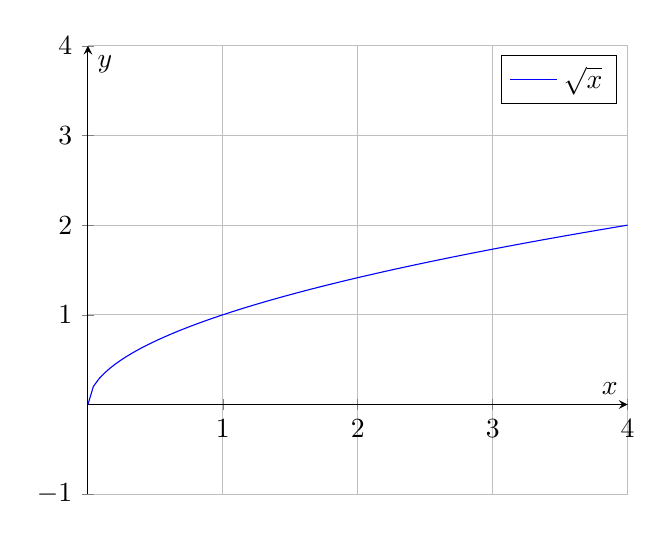
\begin{tikzpicture}
						\begin{axis} [
							axis lines=middle,
							grid,
							ymin=-1,
							ymax=4,
							xlabel={$x$},
							ylabel={$y$}
							]
							\addplot [
								domain=0:4,
								color=blue,
								samples=100
							]
							{x^(1/2)};
							
							\addlegendentry{$\sqrt{x}$};
						\end{axis}
					\end{tikzpicture}
				\end{center}
				\newpage
				\textbf{Cube Root Function}
				\[f(x)=\sqrt[3]{x}\;\;\mathbf{or}\;\;f(x)=a\sqrt[3]{x-h}+k\;\;\;\;\mathbf{Point\;of\;inflection\;at\;}(h,k)\]
				\begin{center}
					\begin{tikzpicture}
						\begin{axis} [
							axis lines=middle,
							grid,
							xmin=-5,
							xmax=5,
							ymin=-4,
							ymax=4,
							xlabel={$x$},
							ylabel={$y$}
							]
							\addplot [
							domain=-5:5,
							color=blue,
							samples=100
							]
							{CubeRoot(x)};
							
							\addlegendentry{$\sqrt[3]{x}$}
						\end{axis}
					\end{tikzpicture}
				\end{center}
			\subsubsection{Reciprocal Root Functions}
				\[f(x)=\frac{a}{\sqrt[n]{b(x-h)}}+k\]
				\textbf{Reciprocal Square Root}
				\[f(x)=\frac{1}{\sqrt{x}}\;\;\mathbf{or}\;\;f(x)=\frac{a}{\sqrt{x-h}}+k\;\;\;\;\mathbf{Asymptotes\;at\;}x=h,\;y=k\]
				\begin{center}
					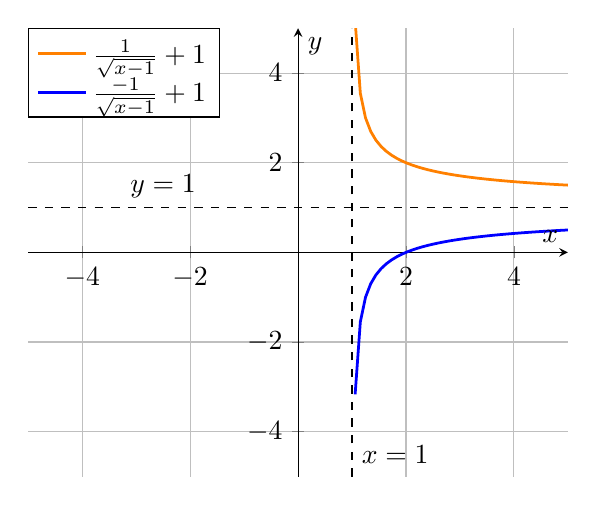
\begin{tikzpicture}
						\begin{axis} [
								axis lines=middle,
								grid,
								xmin=-5,
								xmax=5,
								ymin=-5,
								ymax=5,
								xlabel={$x$},
								ylabel={$y$},
								restrict y to domain=-10:10,
								restrict x to domain=-10:10,
								legend style={at={(0,1)},anchor=north west}
							]
							\addplot [
							domain=-5:5,
							color=orange,
							samples=105,
							line width=1pt
							]
							{(1)/((x-1)^(1/2))+1};
							
							\addlegendentry{$\frac{1}{\sqrt{x-1}}+1$}
							
							\addplot [
							domain=-5:5,
							color=blue,
							samples=105,
							line width=1pt
							]
							{(-1)/((x-1)^(1/2))+1};
							
							\addlegendentry{$\frac{-1}{\sqrt{x-1}}+1$}
							
							\addplot[samples=10,dashed,domain=-5:5] {1}node[above,pos=0.25]{$y=1$};
							\draw[dashed] ({axis cs:1,0}|-{rel axis cs:0,0}) -- ({axis cs:1,0}|-{rel axis cs:0,1})node[right,pos=0.05]{$x=1$};
							
						\end{axis}
					\end{tikzpicture}
				\end{center}
				\newpage
				\textbf{Reciprocal Cube Root}
				\[f(x)=\frac{1}{\sqrt[3]{x}}\;\;\mathbf{or}\;\;f(x)=\frac{a}{\sqrt[3]{x-h}}+k\;\;\;\;\mathbf{Asymptotes\;at\;}x=h,\;y=k\\\]
				\begin{center}
					\begin{tikzpicture}
						\begin{axis} [
							axis lines=middle,
							xmin=-3,
							xmax=3,
							ymin=-3,
							ymax=3,
							ytick={-1,-2,1,2},
							restrict y to domain=-6:6,
							xlabel={$x$},
							ylabel={$y$},
							unbounded coords=jump,
							legend style={at={(0,0)},anchor=south west}
							]
							
							\addplot [very thick, blue, samples=1000, domain=-9:0.999] {1/(CubeRoot(x-1))+1};
							\addlegendentry{$\frac{1}{\sqrt[3]{x-1}}+1$};
							
							\addplot [very thick, red, samples=1000, domain=-9:0.999] {-1/(CubeRoot(x-1))+1};
							\addlegendentry{$\frac{-1}{\sqrt[3]{x-1}}+1$};
							\addplot [very thick, red, samples=1000, domain=0.999:11] {-1/(CubeRoot(x-1))+1};
							\addplot [very thick, blue, samples=1000, domain=0.999:11] {1/(CubeRoot(x-1))+1};
							
							\addplot[samples=10,dashed,domain=-5:5] {1}node[above,pos=0.25]{$y=1$};
							\draw[dashed] ({axis cs:1,0}|-{rel axis cs:0,0}) -- ({axis cs:1,0}|-{rel axis cs:0,1})node[right,pos=0.05]{$x=1$};
							
						\end{axis}
					\end{tikzpicture}
				\end{center}
			\subsubsection{Rational Power Functions}
				\[f(x)=a[b(x-h)]^\frac{p}{q}\]
				If $p > q$ then the polynomial shape will dominate as $\frac{p}{q}>1$.\newline
				If $p < q$ then the root shape will dominate as $0<\frac{p}{q}<1$.
				\begin{center}
					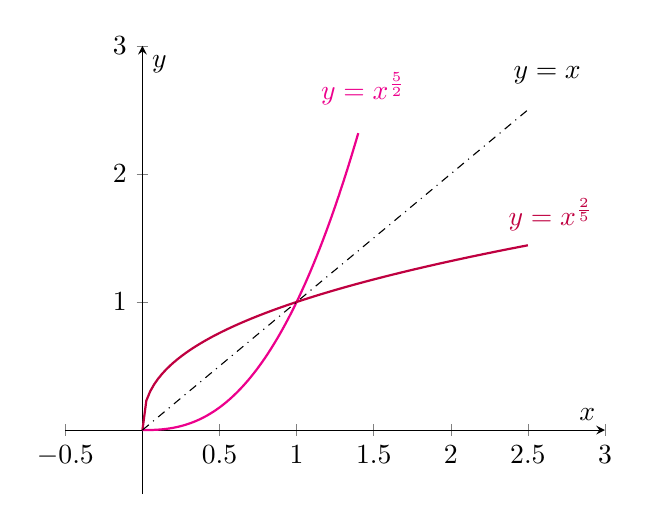
\begin{tikzpicture}
						\begin{axis} [
							axis lines=middle,
							xmin=-0.5,
							xmax=3,
							ymin=-0.5,
							ymax=3,
							xlabel={$x$},
							ylabel={$y$}
							]
							
							\addplot [
								thick, 
								color=magenta, 
								domain=0:1.4, 
								samples=100] 
								{x^(5/2)}
								node[
									above,
									pos=1.05
								]
								{$y=x^\frac{5}{2}$};;
							
							\addplot [
								thick, 
								color=purple, 
								domain=0:2.5, 
								samples=100] 
								{x^(2/5)} 
								node[
									above,
									pos=1.05
								]
								{$y=x^\frac{2}{5}$};
							
							\addplot [
								dashdotted, 
								color=black, 
								thin, 
								domain=0:2.5] 
								{x}
								node[
									above,
									pos=1.05
								]
								{$y=x$};
						\end{axis}
					\end{tikzpicture}
				\end{center}
				\textit{Polynomial Domination ($p > q$)} \newline
				For even values of $p$, the function will be in turning-point form (act like a quadratic or quartic). For odd values of $p$, the function will be in point of inflection form (act like a cubic).
				\newline\newline
				\textit{Root Domination ($p < q$)} \newline
				For even values of $p$, the function with exhibit square-root-like behaviour. For odd values of $p$, the function will exhibit cube-root-like behaviour.\newline\newline
				\textbf{Negative Rational Power Functions}
				\[f(x)=a[b(x-h)]^{-\frac{p}{q}}\]
				\begin{center}
					\bgroup
					\def\arraystretch{1.5}
					\begin{tabular}{|c|}
						\hline
						If $p > q$ the negative power shape dominates as $-\frac{p}{q}<-1$.\\
						\hline
						If $p < q$ the reciprocal root shape dominates as $-1<-\frac{p}{q}<0$.\\
						\hline
						If $p = q$ then $y=\frac{1}{x}$.\\
						\hline
						As $\frac{p}{q}\to1$ the graph of $x^\frac{p}{q}\to\frac{1}{x}$ and approaches a hyperbola.\\
						\hline
					\end{tabular}
					\egroup
				\end{center}
				\textit{Domain}\newline
				For even values of $q$ the domain is $(h,\infty)$ for $b>0$ and $(-\infty,h)$ for $b<0$.\newline
				For odd values of $q$ the domain is $\mathbb{R}\setminus\{h\}$.
				\newline\newline
				For even values of $p$, the function will exhibit truncus-like behvaiour. For odd values of $p$, the function will exhibit hyperbola-like behaviour.
			\subsubsection{Exponential and Natural Log Functions (Euler's Number)}
				\textbf{Euler's Number}\newline
				Compound growth is a repeated percentage increase. That is, multiplying a number by $(1+r\%)$ over and over. If we assume 100\% growth we get $(1+\frac{1}{n})^n$. If we increase the number of successive compoundings to infinity we get the following limit:
				\[\lim_{x\to\infty}\left(1+\frac{1}{n}\right)^n\approx2.71828\]
				This is what we call $e$ or Euler's number. $e$ is the maximum proportion of growth when we compound at 100\% as much as possible.\newline\newline
				\textbf{General Exponential Function}
				\[f(x)=a^x,\;\;\;a\in\mathbb{R}^+\]
				\[f(x)=Aa^{n(x-b)}+c,\;\;\;a\in\mathbb{R}^+\]
				\textit{Range and Domain}\newline
				$x\in\mathbb{R}$\newline
				$y\in(c,\infty),\;\;\;A>0$\newline
				$y\in(-\infty,c),\;\;\;A<0$\newline
				\newpage
				\noindent\textbf{Natural Exponential Function}
				\[f(x)=e^x,\;\;\;e\approx2.71828\]
				\[\int e^xdx = e^x + c \;\;\;\; \frac{d}{dx}(e^x)=e^x\]
				Since we do not always compound at 100\% we need to modify $e$ accordingly. By taking a power of $e$ we can use it to modify the rate or the time or both of compounding. $e^x$ can be interpreted as:
				\begin{itemize}
					\item the proportion of growth after $x$ time periods with 100\% continuous growth, or
					\item the proportion of growth with a continuous rate of $x$ in one time period, or
					\item the proportion of growth where $x=rate\times time$.
				\end{itemize}
				\textbf{General Logarithm Functions}
				\[f(x)=\log_a(x),\;\;a>1\]
				\[f(x)=A\log_a(n(x-b))+c,\;\;a>1\]
				\textit{Range and Domain}\newline
				$x\in(0,\infty)$ for $n>0$\newline
				$x\in(-\infty,0)$ for $n<0$\newline
				$y\in\mathbb{R}$\newline\newline
				\textbf{Natural Logarithm Function, $\log_e(x)$}\newline
				Logarithms are the index of a power. Therefore, the natural logarithm is the index of the natural exponential. The natural logarithm can thus be determined as:
				\begin{itemize}
					\item the time taken to reach a certain proportion of growth with a 100\% continuous growth rate, or
					\item the continuous rate needed to reach a certain proportion of growth in one unit of time, or
					\item the product of the time and the continuous rate.
				\end{itemize}
				More specifically, we can use the natural logarithm to convert to continuous growth rates:
				\[growth=a^{time}=\left(e^{\log_e(a)}\right)^{time}=\left((e^{rate})^{time}\right)=e^x,\;\;\;\;\log_e(e^x)=x\]
				\[growth=a^{rate}=\left(e^{\log_e(a)}\right)^{rate}=\left((e^{time})^{rate}\right)=e^x,\;\;\;\;\log_e(e^x)=x\]
				\newpage
			\subsubsection{Circular Functions}
				\textbf{Sine and Cosine Functions}
				\[f(x)=\sin(x)\;\;\mathbf{or}\;\;f(x)=a\sin(n(x-b))+c\]
				\[f(x)=\cos(x)\;\;\mathbf{or}\;\;f(x)=a\cos(n(x-b))+c\]
				\textit{Period}\newline
				The period of $\sin(nx)$ and $\cos(nx)$ is given by $\frac{2\pi}{n}$.\newline\newline
				\textit{Stationary Points}\newline
				Sine and cosine have a maximum of +1 and minimum values of -1. These values will change under transformations as outlined in the general forms above. The maximums and minimums can be determined as follows: \newline
				\bgroup
				\def\arraystretch{1.5}
				\begin{center}	
					\begin{tabular}{|c|c|}
						\hline
						Maximum & Minimum \\
						\hline
						$c+a$ for $a>0$ & $c-a$ for $a>0$ \\
						\hline
						$c-a$ for $a<0$ & $c+a$ for $a<0$ \\
						\hline
					\end{tabular}
				\end{center}
				\egroup
				\noindent\textit{Sketching Sinusoidal Curves}\newline
				To sketch a sine or cosine function, sketch the minimum, mean and maximum values at 4 points. For $\sin(x)$ or $\cos(x)$ we use $(0,\frac{\pi}{2},\pi,\frac{3\pi}{2},2\pi)$.\newline\newline
				\underline{VCAA 2004 Exam 1 Question 4a}\newline
				On the set of axes, sketch the graph of the function with rule $y=3\sin\left(2\left(t-\frac{\pi}{4}\right)\right),-\pi\le t\le\pi$.\newline
				\bgroup
				\def\arraystretch{1.5}
				\begin{tabular}{|c|c|c|c|c|c|}
					\hline
					$\theta=2\left(t-\frac{\pi}{4}\right)$ & 0 & $\frac{\pi}{2}$ & $\pi$ & $\frac{3\pi}{2}$ & $2\pi$ \\
					\hline
					$t-\frac{\pi}{4}$ & 0 & $\frac{\pi}{4}$ & $\frac{\pi}{2}$ & $\frac{3\pi}{4}$ & $\pi$ \\
					\hline
					$t$ & $\frac{\pi}{4}$ & $\frac{\pi}{2}$ & $\frac{3\pi}{4}$ & $\pi$ & $\frac{5\pi}{4}$ \\
					\hline
					$\sin(\theta)$ & 0 & 1 & 0 & -1 & 0 \\
					\hline
					$3\sin(\theta)$ & 0 & 3 & 0 & -3 & 0 \\
					\hline
				\end{tabular}\hfill
				\egroup
				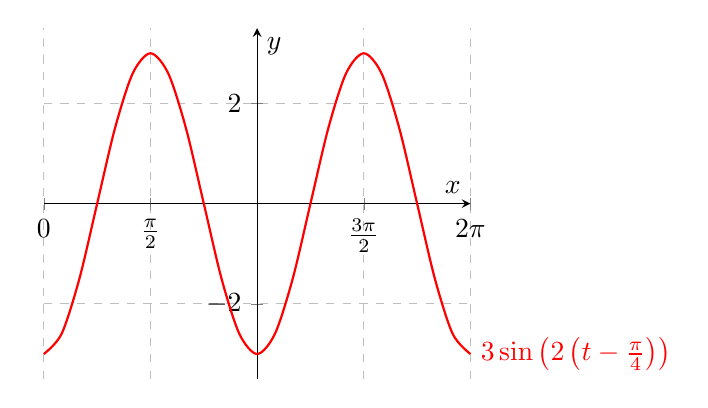
\begin{tikzpicture}[baseline=(current axis.outer west)]
					\begin{axis}[
						xmin=-pi,
						clip=false,
						xmax=pi,
						ymax=3.5,
						ymin=-3.5,
						axis lines=middle,
						xlabel=$x$,
						ylabel=$y$,
						trig format plots=rad,
						grid,
						grid style={dashed},
						xtick={-pi,-pi/2,0,pi/2,pi},
						xticklabels={$0$, $\frac{\pi}{2}$, $\pi$, $\frac{3\pi}{2}$, $2\pi$},
						width={7cm}	
						]
						
						\addplot [color=red, thick, smooth, domain=-pi:pi] {3*sin(2*(x-(pi/4)))} node[right,pos=1]{$3\sin\left(2\left(t-\frac{\pi}{4}\right)\right)$};
						
					\end{axis}
				\end{tikzpicture}
				\textit{Graph Equivalence}\newline
				The graph of cosine is:
				\begin{itemize}
					\item reflection in the y-axis and translation of $\frac{\pi}{2}$ units right of the graph of the sine.
					\item reflection in the x-axis and translation of $\frac{\pi}{2}$ units right of the graph of the sine.
					\item translation of $\frac{\pi}{2}$ units left of the graph of the sine.
				\end{itemize}
				\newpage
				\noindent\textbf{The Tangent Function}
				\[f(x)=\tan(x)\;\;\mathbf{or}\;\;f(x)=a\tan(n(x-b))+c\]
				\textit{Period}\newline
				The period of $\tan(x)$ is $\pi$. For $\tan(nx)$, the period is given by $\frac{\pi}{2}$.\newline\newline
				\textit{Domain and Asymptotes}\newline
				Since $\tan(x)=\frac{\sin(x)}{\cos(x)}$, $\tan(x)$ is undefined whenever $\cos(x)$ is also undefined. $\tan(nx)$ is undefined at $x=\frac{\pi}{2n}$. These are the asymptotes of the function and their x-coordinates can be found by adding and subtracting $\frac{\pi}{n}$ to/from $\frac{\pi}{2n}$.
				\newline
				\newline
				The domain can be written using unions of each period of the tangent, or using set rejection. For $0\le x\le2\pi$, the domain of $\tan(x)$ is $\left[0,\frac{\pi}{2}\right)\cup\left(\frac{\pi}{2},\frac{3\pi}{2}\right)\cup\left(\frac{3\pi}{2},2\pi\right]$ or $[0,2\pi]\setminus\set{\frac{\pi}{2},\frac{3\pi}{2}}$. A similar process can be followed for the domain of $\tan(nx)$.
				\newline\newline
				\textit{Stationary Points}\newline
				There are no stationary points for tangent functions. There is a point of inflection but it is not stationary (not horizontal, i.e. gradient at point of inflection is $\ne$ 0).\newline\newline
				\noindent\textit{Sketching Tangent Graphs}\newline
				To sketch a tangent function, we use the angles where the tangent is horizontal or vertical on the unit circle $(-\frac{\pi}{2},0,\frac{\pi}{2})$ and their related tangent values (0 and undefined) as well as $\pm\frac{\pi}{4}$ for another point to use as a scale between the zeroes and asymptotes whose tangents are $\pm1$.\newline\newline
				\underline{VCAA 2017 NHT Exam 1 Question 4a}\newline
				Let $f:\left[-\frac{\pi}{2},\frac{\pi}{2}\right]\to\mathbb{R},$ where $f(x)=\tan(2x)+1$. Sketch the graph of $f$ on the axes below. Label any asymptotes with the appropriate equation, and label the end points and the axis intercepts with their coordinates.\newline
				\bgroup
				\def\arraystretch{1.5}
				\begin{tabular}{|c|c|c|c|c|c|}
					\hline
					Angle: $2x$ & $-\frac{\pi}{2}$ & $-\frac{\pi}{4}$ & 0 & $\frac{\pi}{4}$ & $\frac{\pi}{2}$ \\
					\hline
					$x$ & $-\frac{\pi}{4}$ & $-\frac{\pi}{8}$ & 0 & $\frac{\pi}{8}$ & $\frac{\pi}{4}$ \\
					\hline
					$\tan(2x)$ & Undefined & -1 & 0 & 1 & Undefined \\
					\hline
					$\tan(2x)+1$ & Undefined & 0 & 1 & 2 & Undefined \\
					\hline
				\end{tabular}\hfill
				\egroup
				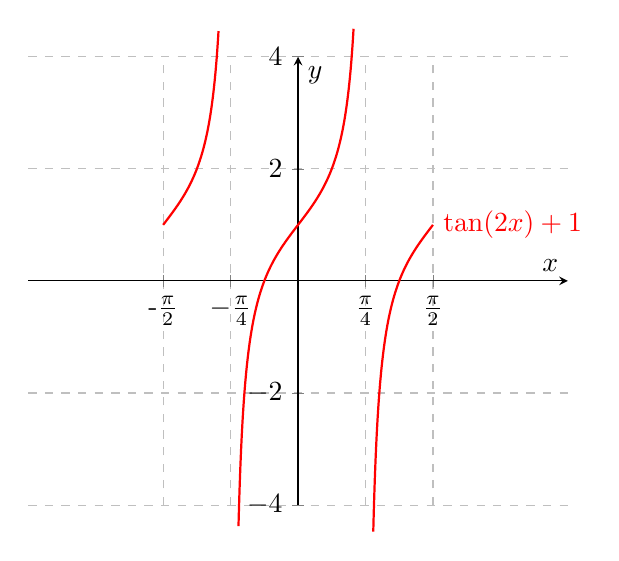
\begin{tikzpicture}[baseline=(current axis.outer west)]
					\begin{axis}[
						xmin=-pi,
						clip=false,
						xmax=pi,
						ymax=4,
						ymin=-4,
						restrict y to domain=-4.5:4.5,
						axis lines=middle,
						xlabel=$x$,
						ylabel=$y$,
						trig format plots=rad,
						grid,
						grid style={dashed},
						xtick={-pi/2,-pi/4,0,pi/4,pi/2},
						xticklabels={-$\frac{\pi}{2}$,$-\frac{\pi}{4}$,0,$\frac{\pi}{4}$,$\frac{\pi}{2}$}
						]
						
						\addplot [color=red, thick, smooth, domain=-0.5*pi:0.5*pi, samples=1000] {tan(2*x)+1} node[right,pos=1]{$\tan(2x)+1$};
						
					\end{axis}
				\end{tikzpicture}
			\subsubsection{Sum and Difference Functions}
				Sum and difference functions are functions that are comprised of basic functions added or subtracted from each other. Polynomials are the sum and difference of power functions with positive integer powers.\newline\newline
				\textbf{Sum Functions}\newline
				The ordinates, or y-values, of a sum function are defined as the sum of the ordinates of the constituent functions. The domain of a sum function is defined as the set of x-values over which both functions are defined.\newline
				\[(f+g)(x)=f(x)+g(x),\;\;d_{f+g}=d_f\cap d_g\]
				\noindent\textbf{Difference Functions}\newline
				Difference functions can be written as a sum function with the reflection of the function in the x-axis.\newline
				\[(f-g)(x)=f(x)-g(x)=f(x)+(-g(x)),\;\;d_{f-g}=d_f\cap d_g\]
				\underline{VCAA 2013 Exam 2 Question 5}\newline
				If $f:(-\infty,1)\to\mathbb{R},f(x)=2\log_e(1-x)$ and $g:[-1,\infty)\to\mathbb{R},g(x)=3\sqrt{x+1}$, find the maximal domain of (f+g)(x).\newline\newline
				The maximal domain of the function $(f+g)(x)$ is $d_f\cap d_g=(-\infty,1)\cap[-1,\infty)=[-1,1)$
				\newline\newline
				\textbf{Sketching Sum and Difference Functions}\newline
				To sketch the graph of a sum or difference function, we add the ordinates (y-values) of each coordinate from both graphs together. We can speed up this process by applying some generalisations:\newline
				\begin{itemize}
					\item The sum function will have an x-intercept when the two functions have the same value but with opposite signs.
					\item If one graph has an x-intercept, then the sum function's ordinate will equal the other function's at that point.
					\item If either graph has a vertical asymptote, the sum function will also have that asymptote.
				\end{itemize}
			\subsubsection{Product Functions}
				Product functions consist of basic functions multiplied together. Polynomials are the product of linear and power functions with positive integers.\newline\newline
				The ordinates of a product function are defined as the product of the ordinates of the constituent functions. The domain of the product function is the set of x-values over which both functions are defined.\newline
				\[(fg)(x)=f(x)\times(x),\;\;d_{fg}=d_f\cap d_g\]
				\underline{Modified VCAA 2013 Exam 2 Question 5}\newline
				If $f: (-\infty,1)\to\mathbb{R},f(x)=2\log_e(1-x)$ and $g: [-1,\infty)\to\mathbb{R},g(x)=3\sqrt{x+1}$, find the maximal domain of the product function $(fg)(x)$.\newline\newline
				The maximal domain of the function $(fg)(x)$ is $d_f\cap d_g = (-\infty,1)\cap[-1,\infty)=[-1,1)$.\newline\newline
				\textbf{Sketching Product Functions}\newline
				The ordinates of a product function can be found by taking the product of the ordinates of the two constituent functions. This can be expedited via some generalisations like the sum and difference functions:\newline
				\begin{itemize}
					\item The product function has an x-intercept when either function has an x-intercept.
					\item If one function's ordinate is 1, the product function's ordinate equals the other function's at that point.
					\item If one function's ordinate is -1, the product function's ordinate equals the opposite of the other function's ordinate at that point.
					\item If the two graphs are both positive or both negative, the product function will be positive.
					\item If the two graphs have different signs, the product function will be negative.
				\end{itemize}
			\subsubsection{Composite Functions}
				Composite functions are the result of nesting a function inside another. The notation for this is below.
				\[f\circ g(x)=f(g(x)),\;\;d_{f\circ g}=d_g \setminus {x:g(x)\notin d_f},\;\;r_g\subset d_f\]
				\textbf{Effect of the Outside Function $f(x)$}\newline
				The outside function gives the general shape of the graph of the composite function. That is, $f(x)$ determines the general shape of the graph $y=f(g(x))$.\newline\newline
				\textbf{Effect of the Inside Function $g(x)$}\newline
				The inside function gives the sections of the outside function to graph.\newline
				For $g(x)>0$, the graph of $y=f(g(x))$ is similar to the graph of $y=f(x)$ on the right of the y-axis.\newline
				For $g(x)<0$, the graph of $y=f(g(x))$ is similar to the graph of $y=f(x)$ on the left of the y-axis.\newline\newline
				The smaller the value of $g(x)$, the graph of $y=f(g(x))$ is similar to $y=f(x)$ closer to the y-axis and vice-versa.\newline\newline
				If $g(x)$ is sine, cosine, or tangent, the graph of $y=f(g(x))$ will loop horizontally.\newline
				If $g(x)$ is an even function ($g(x)=g(-x)$), then $f(g(x))$ will also be an even function.\newline
				If $g(x)$ has an asymptote at $x=a$, then the graph of $y=f(g(x))$ will also have an asymptote at $x=a$.\newline\newline
			\subsubsection{Piecewise Functions}
				A piecewise function is a function that takes the shape of different functions in different sections of its domain.\newline
				\[
					f(x)=\begin{cases}
						x^2 & x\leq 0\\
						\frac{100-x}{100} & 0<x\leq 100 \\
						2x+1 & 100<x
					\end{cases}
				\]
		\subsection{Transformations of the Plane and Functions}
			\subsubsection{Transformations of the Plane}
				In geometry, we can transform shapes (and the plane) by using transformations. Three such transformations are dilations (enlargement or shrinking), reflections (mirror across a line), and translations (sliding). In Coordinate Geometry, the same transformations can be applied to points and graphs.
				\newline\newline
				\textit{Dilations}\newline
				Dilations involve multiplying the x or y values by a scaling factor. That is, stretch it in a direction by a factor (e.g. dilated in the y-direction by a factor of 2).
				\newline\newline
				Dilations can be either phrased as:
				\begin{itemize}
					\item dilation by a factor of $a$ in the $x/y$ direction, or
					\item dilation by a factor of $a$ away from the $y/x$ axis.
				\end{itemize}
				\textit{Reflections}\newline
				Reflections involve multiplying the x or y values by a negative. By multiplying the x-value by a negative, the number reflects in the y-axis. By multiplying the y-value by a negative, reflection in the x-axis occurs.
				\newline\newline
				\textit{Translations}
				Translations involve adding a number to the x or y values. That is, moving every point uniformally by the same amount in the same direction.
			\subsubsection{Constructing a Function from a List of Transformations}
				To transform a function from a given list of transformations, we can apply all the the transformations to each point on the graph by applying them generally to x and y then modify the function accordingly.
				\newline\newline
				Since the transformations are based on multiplication and addition, the order of operations needs to be considered.
				\newline
				For the function $y=f(x)$ we can see there is a $y=$ term, so vertical transformations can be applied directly to the function. That is, the new $y,\;y'=ay+d=af(x)+d$.
				\newline
				However, there is no $x=$ term, so the horizontal transformations need to be rearranged to substitute into the original x. That is, for the new $x,\;x'=bx+c$, we need to rearrange to $x=\frac{1}{b}(x'-c)$.
				\newpage
				\noindent\underline{VCAA 2002 Exam 1 Question 5a}\newline
				The graph of the function with rule $y=\frac{1}{x}$ is transformed as follows:
				\begin{itemize}
					\item a dilation by a factor of $\frac{1}{2}$ from the y-axis
					\item a reflection in the y-axis
					\item a translation of +3 units parallel to the x-axis
					\item a translation of +1 unit parallel to the y-axis
				\end{itemize}
				Find the equation of the rule of the transformed function.
				\[(x,y)\to\left(\frac{1}{2}x,y\right)\to\left(-\frac{1}{2}x,y\right)\to\left(-\frac{1}{2}x+3,y\right)\to\left(-\frac{1}{2}x+3,y+1\right)=(x',y')\]
				\[x'=-\frac{1}{2}x+3\implies x=-2(x'-3)\]
				\[y'=y+1=\frac{1}{x}+1=\frac{1}{-2(x'-3)}+1\implies y=\frac{1}{-2(x-3)}+1\;\;\text{is the transformed function.}\]
			\subsubsection{Describing the Effect of Transformations}
				When a function has been transformed, the x and y values have been manipulated in some manner. It is useful to describe these transformations specifically as it makes sketching graphs of transformed functions much easier.
				\newline\newline
				\underline{VCAA 2009 Exam 2 Question 12}\newline
				A sequence of transformations that maps the curve $y=\sqrt{x}$ to the curve $y=1-3\sqrt{2x+\pi}$ is...\newline
				$\text{let}\; y'=1-3\sqrt{2x'+\pi}=1-3\sqrt{x}=-3\times y + 1$
				$x=2x'+\pi \implies x'=\frac{1}{2}x-\frac{\pi}{2}$
				Hence it is evident that the order of transformations is:
				\begin{itemize}
					\item Dilation by a factor of 3 from the x-axis
					\item Dilation by a factor of $\frac{1}{2}$ from the y-axis
					\item Reflection in the x-axis
					\item Translation of 1 unit up and $\frac{\pi}{2}$ units left
				\end{itemize}
			\newpage
			\subsubsection{Inverse Transformations}
				If you are able to transform $y=f(x)\to y=Af(n(x-h))+k$ then inverse transformations reverse the process. Inverse transformations must be applied in the reverse order to that in which they were originally applied.
				\newline\newline
				\bgroup
				\def\arraystretch{1.5}
				\begin{tabular}{|c|c|}
					\hline
					Transformation & Inverse Transformation \\
					\hline
					Dilation by a factor of $A$ parallel to y-axis & Dilation by a factor of $\frac{1}{A}$ parallel to the y-axis \\
					\hline
					Dilation by a factor of $A$ from the x-axis & Dilation by a factor of $\frac{1}{A}$ from the x-axis \\
					\hline
					Dilation by a factor $n$ parallel to the x-axis & Dilation by a factor $\frac{1}{n}$ parallel to the x-axis. \\
					\hline
					Dilation by a factor $n$ from the y-axis & Dilation by a factor $\frac{1}{n}$ from the y-axis. \\
					\hline
					Reflection in an axis & Reflection in the same axis \\
					\hline
					Translation of $h$ units in positive x-direction & Translation of $h$ units in negative x-direction. \\
					\hline
					Translation of $k$ units in positive y-direction & Translation of $k$ units in negative y-direction. \\
					\hline
				\end{tabular}
				\egroup
			\subsubsection{Equivalent Transformations}
				Since functions can be algebraically manipulated, it is possible to show that different transformations will have the same result for particular graphs. These do not necessarily apply to all functions and different transformations are equivalent for different functions.
				\newline\newline
				\underline{Examples}\newline
				$y=(3x)^2=9x^2$\newline
				Dilation by a factor of $\frac{1}{3}$ from the y-axis is equivalent to a dilation by a factor of 9 from the x-axis.\newline\newline
				$y=(3x)^3=27x^3$\newline
				Dilation by a factor of $\frac{1}{3}$ from the y-axis is equivalent to a dilation by a factor of 27 from the x-axis.\newline\newline
				$y=3x$\newline
				Dilation by a factor of $\frac{1}{3}$ from y-axis is equivalent to a dilation by a factor of 3 from the x-axis.\newline\newline
				$y=\log_3(x)-2=\log_3(\frac{x}{9})$\newline
				Translation 2 units down is equivalent to a dilation by a factor of 9 from the y-axis.\newline\newline
				$y=\log_2(x)+3=\log_2(8x)$\newline
				Translation of 3 units up is equivalent to a dilation by a factor of $\frac{1}{8}$ from the y-axis.\newpage
			\subsubsection{Monoparametric Transformations}
				\textbf{Dilations}
				\[y=Af(x)\]
				"A dilation by a factor of A from the x-axis" or "a dilation by a factor of A parallel to the y-axis". The x-intercepts do not change.\newline
				\[y=f(nx)\]
				"A dilation by a factor of $\frac{1}{n}$ from the y-axis" or "a dilation by a factor of $\frac{1}{n}$ parallel to the x-axis". The y-intercepts don't change.\newline\newline
				\textbf{Reflections}
				\[y=-f(x)\]
				"A reflection in the x-axis."\newline
				Intersections between the original function and its reflection occur on the x-axis.\newline
				\[y=f(-x)\]
				"A reflection in the y-axis."\newline
				Intersections between the original function and its reflection occur on the y-axis.\newline\newline
				\textbf{Translations}
				\[y=f(x)+c\]
				"A translation of $c$ units up (for $c > 0$)" or "a translation of $c$ units down (for $c < 0$)".\newline
				Shape of the curve does not change.\newline
				\[y=f(x+b)\]
				"A translation of $b$ units left (for $b > 0$)" or "a translation of $b$ units right (for $b < 0$)".\newline
				Shape of the curve does not change.\newline
		\subsection{Applications of Functions}
			\subsubsection{Modelling Data and Practical Situations}
				When we collect a set of data, we often want to describe as accurately as possible a function that could generate the same points or at least a good approximation of them. To do this, we need to know what shape the points take, which is best achieved by plotting the data. If the shape is recognisable, we can fit a model to the data easily but some datasets require a combination (sum, difference, or product) of functions to more accurately describe the data.
				\newline\newline
				\textbf{Features that Enable the Recognition of Possible Models}\newline
				\bgroup
				\def\arraystretch{2}
				\begin{tabular}{|c|m{10cm}|}
					\hline
					Positive Power Model $y=ax^n$ & Proportional to the n-th power. \\
					\hline
					Negative Power Model $y=\frac{a}{x^n}$ & Inversely proportional to the n-th power (exhibits asymptotic behaviour). \\
					\hline
					Linear Model $y=mx+b$ & Constantly increasing or decreasing \\
					\hline
					Polynomial Model & Takes the shape of a polynomial \\
					\hline
					\makecell{Sinusoidal Model \\ $y=a\sin(bx)$ or $y=a\cos(bx)$} & Oscillation between two values \\
					\hline
					\makecell{Exponential Model \\ $y=ae^{bx}$} & Increasing or decreasing exponentially (decreasing has asymptotic behaviour) \\
					\hline
					\makecell{Logarithmic Model \\ $y=a\log_e(bx)$} & Slow growth or decay, or data ranges over orders of magnitude. \\
					\hline
				\end{tabular}
				\egroup
			\subsubsection{Applications of Exponential Functions}
				\[A(t)=A_0\times a^{kt}+C\]
				\begin{center}
					\bgroup
					\def\arraystretch{1.5}
					\begin{tabular}{|c|c|}
						\hline
						Modelling Growth if $a>1$ and $k>1$ & Modelling Decay if $0<a<1$ or $k<0$ \\
						\hline
						Cell Growth & Radioactive Decay \\
						\hline
						Population Growth & Population Decay \\
						\hline
						Compound interest & Cooling temperatures \\
						\hline
					\end{tabular}
					\egroup
				\end{center}
				\noindent\textbf{Initial Value}\newline
				The initial value occurs when $t=0$. That is, $A(0)=A_0 + C$.\newline\newline
				\textit{Example}\newline
				A population, $P$, after $t$ years is modelled by $P(t) = 100\times 1.5^t + 20$. The initial population was $P(0)=100\times1.5^0+20=100+20=120$.\newline\newline
				\textbf{Rate of Growth/Decay}\newline
				The rate of growth or decay is the base of the exponential. A multiplier in the index changes the frequency with which the rate is applied. For $e^{bx}$, the continuous rate is $b$.\newline\newline
				\textit{Example}\newline
				An investment is compounding annually such that the amount of the investment $\$A$, after $t$ years is given by $A(t)=5000\times1.067^t$. $A(0)=5000$. The interest rate of the investment is $1+r\% = 1.067 \implies r\%=0.067=6.7\%$.\newline\newline
				\textbf{Half-Life}\newline
				The time it takes for there to be half of the initial value due to a decaying model. That means solving the following:
				\[
					\frac{A_0+C}{2}=A_0\times a^{kt}+C\implies a^{kt}=\frac{1}{2}\;\text{for}\;t
				\]
				\textit{Example}\newline
				A population of sheep is decaying exponentially. At a particular time, there were 1000 sheep observed. Six months later, 800 sheep remained. Determine a function, $A(t)$, that models the population of the sheep $t$ months after the first observation.
				\begin{gather*}
					A_0=1000,\;\;A=1000\times e^{bt}\\
					800=1000\times e^{6b} \implies e^{6b}=\frac{4}{5} \implies b=\frac{1}{6}\log_e\left(\frac{4}{5}\right)\approx-0.0372 \\
					\therefore A=1000\times e^{-0.0372t}
				\end{gather*}
				The continuous rate at which the population of sheep is decaying is 3.72\%. Determine the half-life of the population.
				\[
				e^{-0.0372t}=0.5 \implies -0.0372t = \log_e(0.5) \implies t=18.63\approx 19 months
				\]
				\textbf{Long-Run Value}\newline
				The Long-run value is the value that a decaying model will approach in the long run. As $t\to\infty$, $A\to C$, the horizontal asymptote.\newline\newline
				\textit{Example}\newline
				A population of wild rabbits is in decline. There is an estimate of 760 rabbits when the decline is first notices, 752 after one day, and 716 after two days. An equation to model the rabbit population is in the form $R(t)=a\times b^t + c$ where $R$ is the number of rabbits after $t$ days. Find the long-run value.\newline
				\begin{gather*}
					790=a\times b^0 + c \implies c=790-a\\
					752=a\times b^1 + c \implies 752=ab+790-a \implies a(1-b)=38\\
					716=a\times b^2 + c \implies 716=ab^2+790-a \implies a(1-b^2)=74\\
					\implies a(1-b)(1+b)=74 \implies 38(1+b)=74 \implies 1+b=\frac{37}{19} \implies b=\frac{18}{19}\approx0.95 \\
					a(1-0.95)=38 \implies a=760,\;\;c=790-760=30 \\
					\therefore R(t)=760\times0.95^t + 30 \\
					\text{In the long run, there is expected to be 30 rabbits left.}
				\end{gather*}
			\subsubsection{Applications of Sine and Cosine Functions}
				\underline{VCAA 2001 Exam 2 Question 1 (modified)}\newline
				The temperature $T$ degrees Celsius in a greenhouse at $t$ hours after midnight for a typical November day is modelled by the formula $T = 25-4\cos(\frac{\pi(t-3)}{12}),\;\text{for}\;0\le t\le 24$. Find the period, amplitude and maximum and minimum temperatures of the greenhouse.\newline\newline
				\textbf{NOTCOMPLETE}\newline
			\subsubsection{Determining the Equation of a Function}
				There are multiple methods to determine a function's equation.
				\begin{itemize}
					\item Directly substitute any known coordinates in to the function with variable parameters to create simultaneous equations to solve.
					\item Directly substitute into a particular form of the function.
					\item Use transformations from the graph of the untransformed function to the given graph.
					\item Use knowledge of the function to determine the parameters.
				\end{itemize}
				\noindent\textit{Example}\newline
				Find the values of $a$ and $b$ such that the graph of $f(x)=ae^{bx}$ passes through the points $(\log_e(32),32)$ and $(\log_e(5),500)$. Then express $f(x)$ in the form $e^{mx+n}$.
	\section*{AOS2 - Algebra, Number, and Structure}
		\subsection{Polynomial Equations}
			\subsubsection{Real Solutions}
				A polynomial with real coefficients of up to degree $n$ will have up to $n$ real solutions.
			\subsubsection{Null Factor Law}
				If $a\times b=0$ then $a=0 \text{and/or} b=0$.\newline
				For the polynomial $P(x)=0$, if you can factorise $P(x)$ you can use the null factor law to solve each factor equal to 0.\newline
				Rational root theorem and factor theorem can be used to factorise polynomials.
			\subsubsection{Quadratic Formula}
				Quadratic equations can be solved in three ways: by factorising using null factor law, by completing the square and solving a power equation, or by using the quadratic formula.\newline\newline
				For a quadratic equation in the form $ax^2+bx+c=0$, the solutions are found by
				\[x=\frac{-b\pm\sqrt{b^2-4ac}}{2a}\]
				\textbf{Quadratic Equations using Substitutions}\newline
				Like factoring, some equations can be rewritten as a quadratic equation and thus solved via quadratic methods.\newline\newline
				\textit{Example}\newline
				\begin{align*}
					(2x+1)^2+5(2x+1)+6=0 \\
					\text{Let}\;y=2x+1 \\
					y^2+5y+6=0 \\
					y=\frac{-5\pm\sqrt{5^2-4(1)(6)}}{2}=\frac{-5\pm 1}{2} \\
					y=2x+1=-\frac{4}{2}=-2\implies2x=-3\implies x=-\frac{3}{2} \\
					y=2x+1=-\frac{6}{2}=-3\implies2x=-4\implies x=-2
				\end{align*}
			\subsubsection{The Discriminant and Number of Solutions}
				The discriminant describes the number and types of solutions a quadratic equation has. $\Delta=b^2-4ac$.\newline
				\bgroup
				\def\arraystretch{1.5}
				\begin{center}
					\begin{tabular}{|c|c|}
						\hline
						Number of Real Solutions & Condition \\
						\hline
						2 & $\Delta>0$ \\
						\hline
						1 & $\Delta=0$ \\
						\hline
						0 & $\Delta<0$ \\
						\hline
					\end{tabular}
				\end{center}
				\egroup
				\noindent If the discriminant is a perfect square (or fraction), then the solutions to the quadratic are \textbf{rational}.
		\subsection{Inequalities}
			\subsubsection{Single-Variable Linear Inequalities}
				\textbf{Solving a Single-Variable Linear Inequality}\newline
				To solve a single-variable inequality, we solve for the pronumeral as we would a linear equation. Similar to linear equations, whatever you do to one side of the inequality must be done to the other side.\newline\newline
				\textit{Example}
				\begin{align*}
					x+5\le2 \\
					x \le -3
				\end{align*}
				\textbf{Sketching a Single-Variable Linear Inequality}\newline
				Once we have solved for the pronumeral we can present it graphically. Single-variable linear inequalities are sketched on a number line.
				\begin{center}
					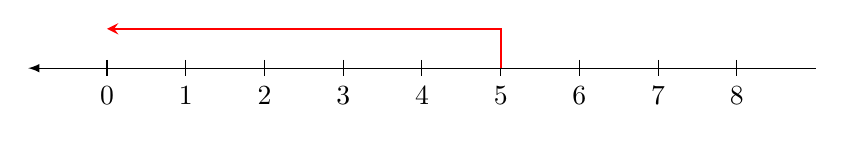
\begin{tikzpicture}
						\draw[latex-] (-1,0) -- (9,0);
						\foreach \x in  {0,1,2,3,4,5,6,7,8} \draw[shift={(\x,0)},color=black] (0pt,3pt) -- (0pt,-3pt);
						\foreach \x in {0,1,2,3,4,5,6,7,8} \draw[shift={(\x,0)},color=black] (0pt,0pt) -- (0pt,-3pt) node[below] {$\x$};
						\draw [red,  thick, -stealth] (5,0) -- ++(0,0.5) -- ++(-5,0);
					\end{tikzpicture}
				\end{center}
		\subsection{Inverse Relations and Functions}
		\subsection{Exponential Equations}
		\subsection{Trigonometric Equations}
		\subsection{Power Equations}
		\subsection{Composite Function Equations}
		\subsection{Solutions to Equations}
		\subsection{Newton's Method}
		\subsection{Equations of the Form $f(x)=g(x)$}
		\subsection{Literal Equations}
		\subsection{Systems of Simultaneous Linear Equations}
	\section*{AOS3 - Calculus}
	\section*{AOS4 - Data analysis, probability, and statistics}
\end{document} 